\chapter{Solidity}

\section{Overview}
\paragraph*{}
Solidity is a relatively new programming language, its first proposal coming in 2014 from the co-founder of Ethereum, Gavin Wood \cite{solidity-lang}. Its purpose is to serve development of smart contracts to be deployed on various blockchain platforms, especially focusing on the Ethereum blockchain.

\paragraph*{}
Although it's been around for around 8 years now, Solidity has just started to peak interest in the blockchain development community. Dune Analytics reported an increase of 75\% in smart contracts deployment in March, 2020, summing up to a total of 2 million smart contracts deployed \cite{coin-telegraph-2020}. Since then, hundreds of thousands of smart contracts have been deployed monthly, with around 370 thousands just in May 2022 \ref{fig:dune-analytics-2022}.

\begin{figure}
    \centering
    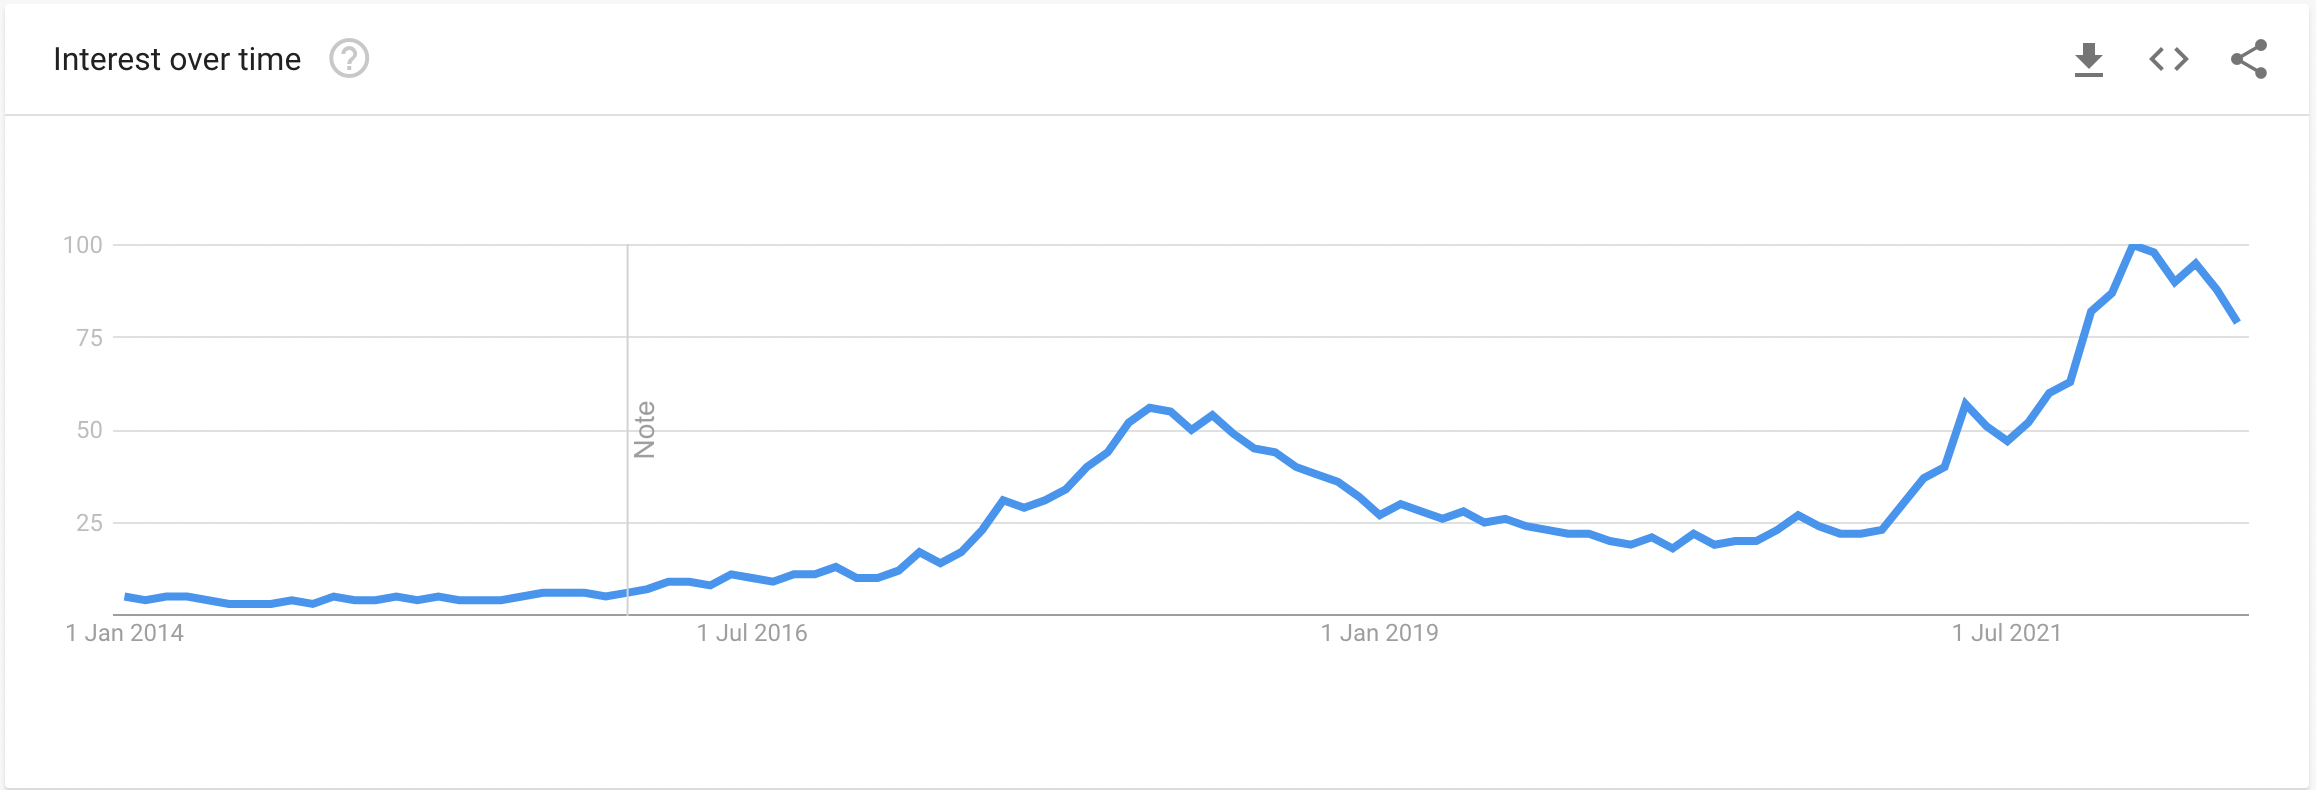
\includegraphics[width=15cm]{images/solidity_interest.png}
    \caption{Solidity interest from 1st of January, 2014, to 1st of June, 2022, according to Google web searches}
    \label{fig:solidity-interest}
\end{figure}

\begin{figure}
    \centering
    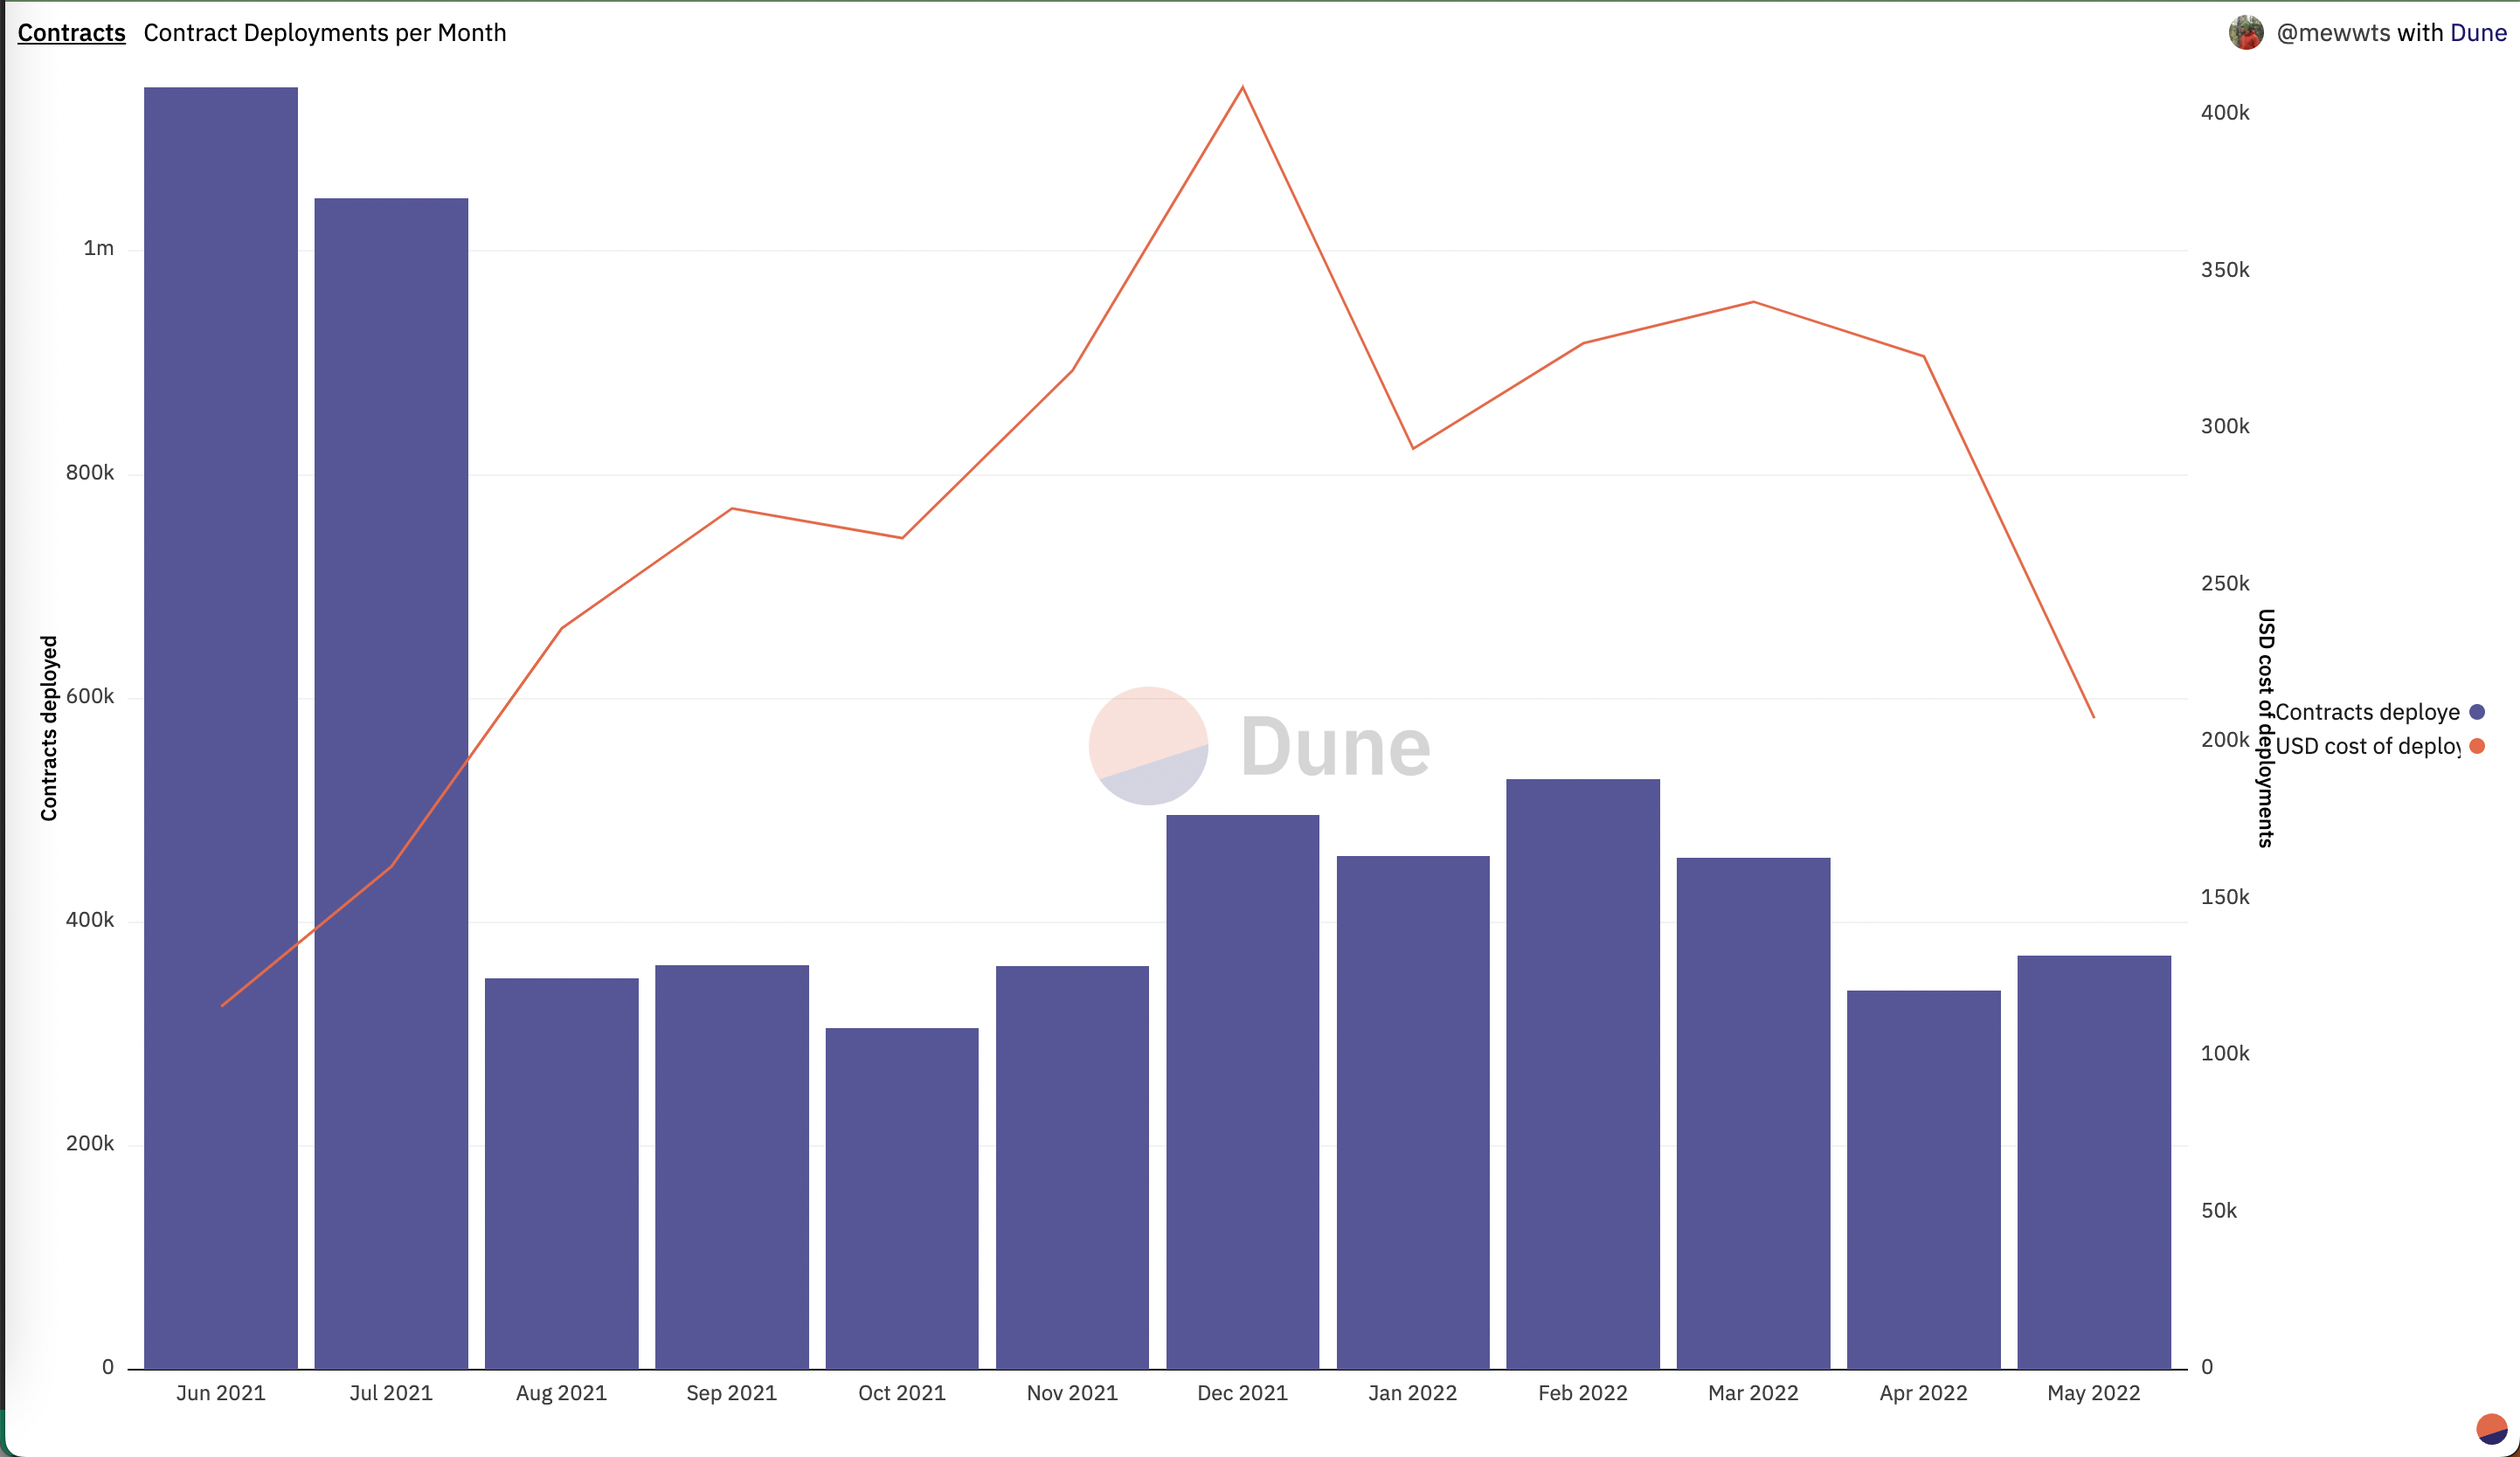
\includegraphics[width=15cm]{images/dune_analytics_2022.png}
    \caption{Contract deployment per month in the past year, according to Dune Analytics}
    \label{fig:dune-analytics-2022}
\end{figure}

\paragraph*{}
The main properties that interests this thesis are that this programming language is \textbf{statically typed} and is converted into bytecode to run inside the Ethereum Virtual Machine (EVM). Being statically typed helps the compiler with static analysis, making possible the development of an optimization suite that performs both common optimizations and particular optimizations for EVM.

\section{Solidity's Compiler and Optimizer}
\paragraph*{}
High level solidity code is sent to \lstinline[columns=fixed]{solc} binary, which stands for ``solidity compiler''. The user may or may not specify the usage of the optimizer with the \lstinline[columns=fixed]{--optimize} flag, which is enabled by default. Upon analyzing the compilation flow \ref*{fig:solc-compilation-flow}, we notice that there are some optional (yet recommended) steps to follow while compiling, which take advantage of Yul (intermediate code representation for Solidity) and Abstract Syntax Trees, the latter being built for both the initial Solidity code and for the Yul IR. If we choose to optimize the code through Yul, then the \lstinline[columns=fixed]{--via-ir} must be specified, which is also enabled by default.

\paragraph*{}
When optimizing through Yul, the compilation flow will actually use \textbf{two optimizers}: the "new" one (Yul optimizer) and the "legacy" one (EVM bytecode optimizer). The reasoning behind this is that bytecode optimization should be as simple and straightforward as possible, this also being an engineering decision made by Solidity's team that they explained in the Solidity Summit presentations, 2022. \lstinline[columns=fixed]{JUMP} instructions are especially tricky to handle while optimizing bytecode, making high level, semantic optimization (for example simplifying \lstinline[columns=fixed]{for} loops) more difficult.

\paragraph*{}
The advantage of having two optimizers is that it decouples work by a great deal. Low level assembly optimizations are done by the legacy optimizer \footnote{Future work might also consist in unifying EVM and LLVM, bringing all of the work and optimization done to LLVM on Solidity's ground as well.}, and more complex optimizations, that require techniques such as data flow analysis, are done directly on the Yul IR, which is later used to generate the efficient bytecode. This also helps to visually inspect the generated Yul IR and making sure that its output is the expected one. Specifically for the team, it means that it makes unit testing and development much easier.

\begin{figure}
    \centering
    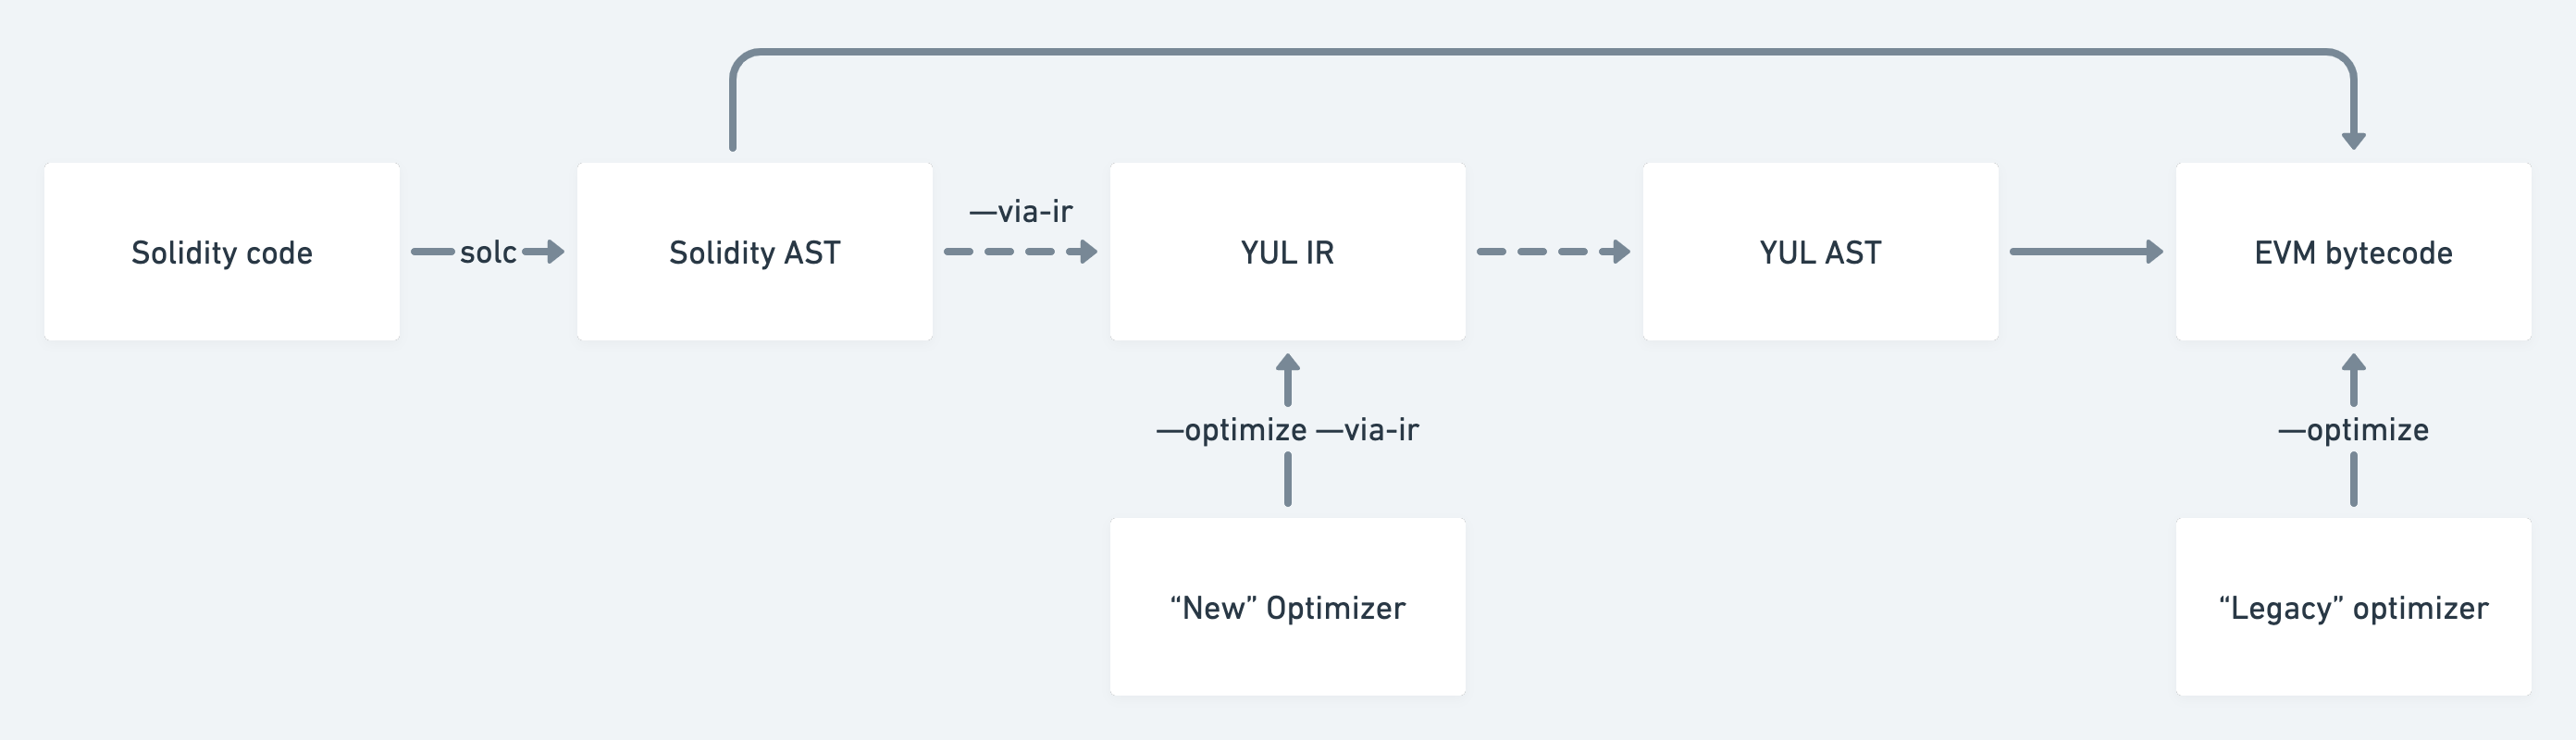
\includegraphics[width=15cm]{images/solc_flow.png}
    \caption{Solidity compilation flow}
    \label{fig:solc-compilation-flow}
\end{figure}

\section{Intermediate Representations}

\subsection*{Abstract Syntax Tree}
\paragraph*{}
\textbf{Abstract Syntax Trees (AST)} are often used to do a first analysis of the code instructions by walking the tree. This is often coupled with the Visitor Design Pattern, where the user implements what the \lstinline[columns=fixed]{visit} function should do for each type of node. They are often used in compilers to represent the structure of the code, to make isolated code changes and then re-generate code from the AST.

\paragraph*{}
Solidity uses ANTLR (ANother Tool for Language Recognition) to generate its AST. On Solidity's territory, ASTs appear in two phases. First, an AST is generated from the unaltered Solidity code, while another AST is later generated from the Yul IR code. The AST nodes provide sufficient granularity to make a structural analysis simple enough, thanks to recursively analysing the children node of a root.

\begin{figure}
    \centering
    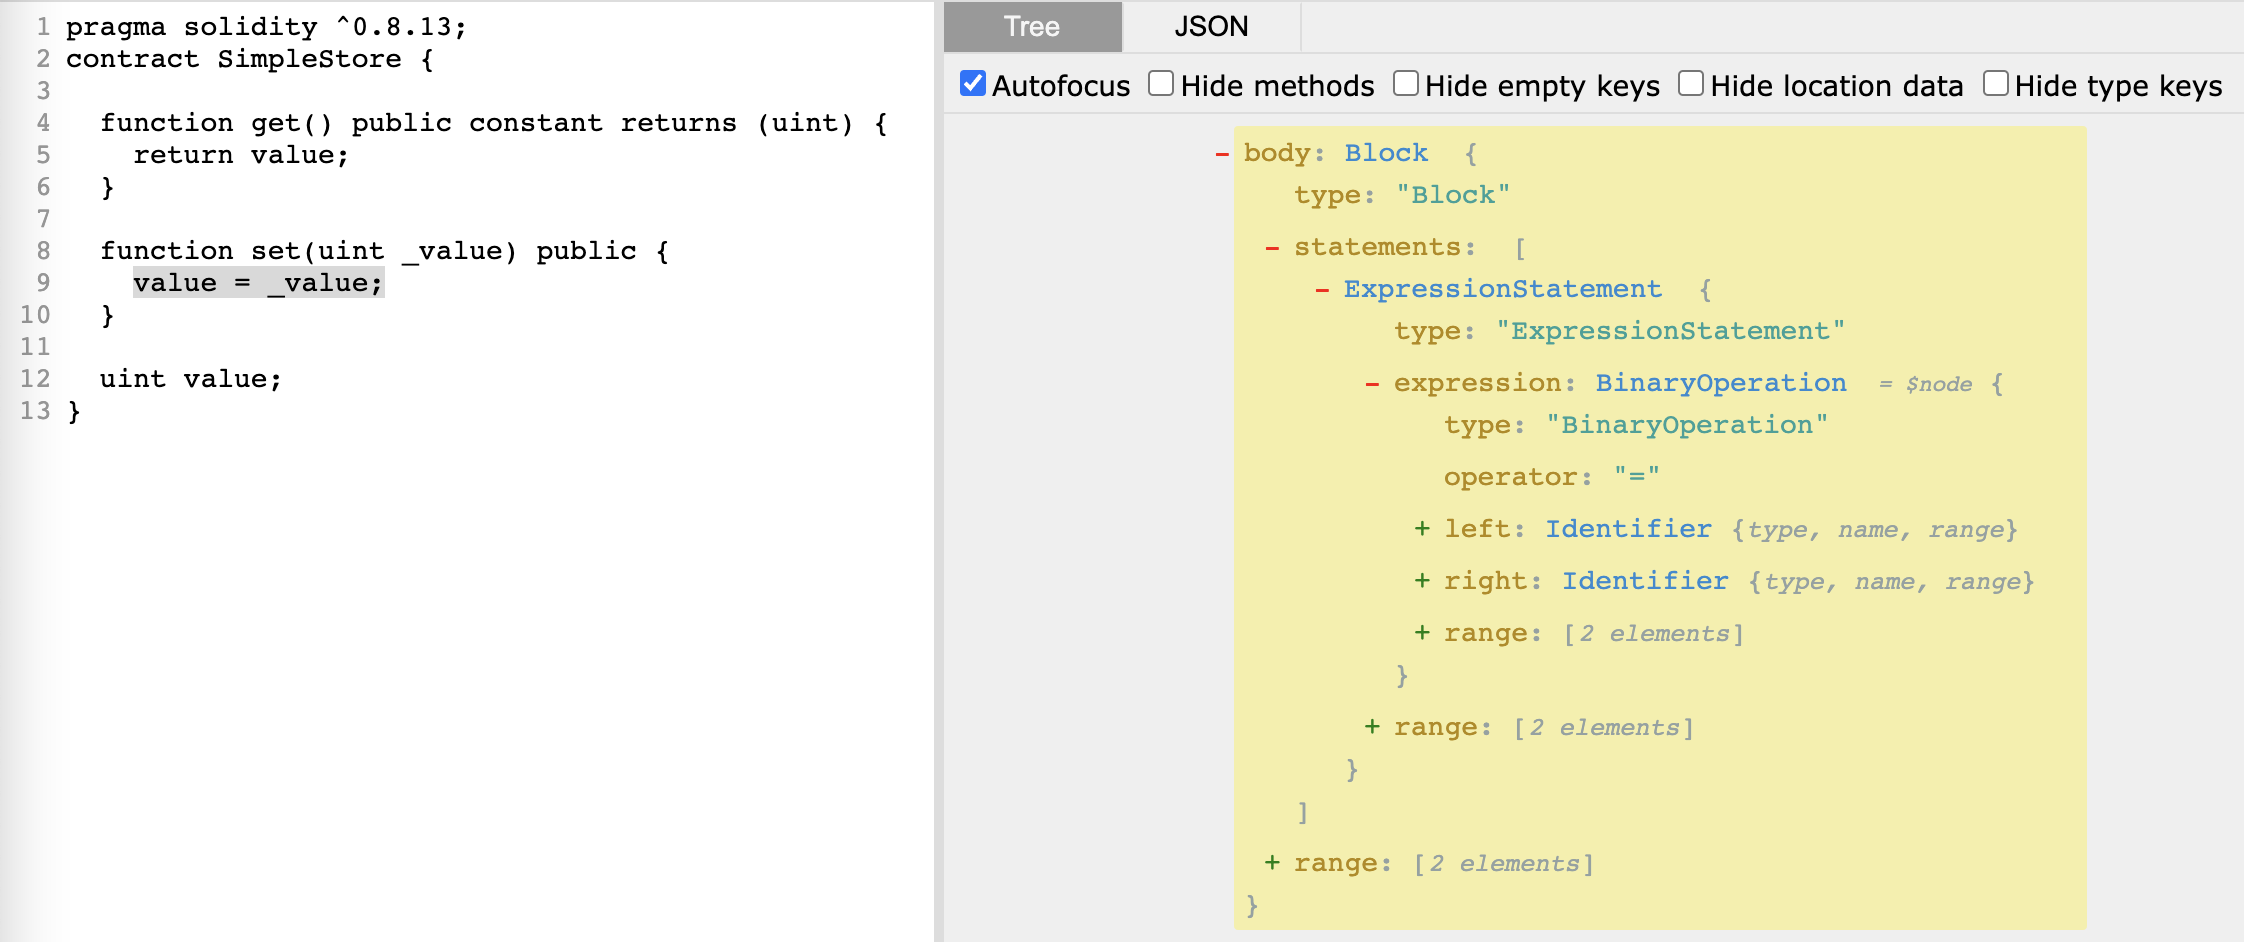
\includegraphics[width=15cm]{images/solidity_ast_example.png}
    \caption{Solidity AST Example. The body of the function is an AST node itself, in which the statements are other AST nodes. Generated using AST Explorer.}
    \label{fig:solidity-ast-example}
\end{figure}

\paragraph*{}
ASTs are very common in static analysis and are often times coupled with a grammar (or dialect) that enforces different node types and node structure in the tree. There are a variety of tools that use ASTs to do code analysis of their own.

% ASTs generated from Solidity code have been used by a variety of tools to inspect code, one of which is Solidity Instrumentation Framework (SIF) \ref{fig:sif-workflow}. The framework builds an internal representation (in C) of the AST nodes, bringing an additional set of features such as symbol renaming or function listing to the table. This works by exposing the \lstinline[columns=fixed]{visit} function to the user, each node being visited with the pattern implemented by the user.


\subsection*{Yul IR}
\paragraph*{}
\textbf{Yul}, former name Julia, is an intermediate representation for Solidity Code. It has been publicly announced as ``production ready'' in March, 2022, in version 0.8.13 of Solidity. Since then, the engineering team has been encouraging people to compile smart contracts via the usage of Yul, since the optimization focus has shifted on this pseudocode language.

\paragraph*{}
Yul was designed around four main principles, as described by its official documentation \cite{yul-description}: readability, easy manual inspection of control flow, simple and straightforward generation of bytecode from Yul and whole-program optimization. As compared to bytecode, this IR provides high-level syntax for instructions that introduce jump instructions (\lstinline[columns=fixed]{JUMP, JUMPDEST, JUMPI}), the reasoning behind this being that it makes analyzing data flow and control flow in the code much easier.

\begin{lstlisting}[caption={Example of Yul code which computes exponentiation recursively}]
{
    function power(base, exponent) -> result
    {
        switch exponent
        case 0 { result := 1 }
        case 1 { result := base }
        default
        {
            result := power(mul(base, base), div(exponent, 2))
            switch mod(exponent, 2)
                case 1 { result := mul(base, result) }
        }
    }
}
\end{lstlisting}

\paragraph*{}
This was designed as an actual programming language, making it possible to generate valid EVM bytecode from Yul code. Of course, it is not recommended to write smart contracts in Yul, but one can do so to get more familiar with the dialect. It also takes on the property of its "parent" code, and is also statically typed as Solidity. This further eases the static analysis done by the compiler.

\begin{figure}
    \centering
    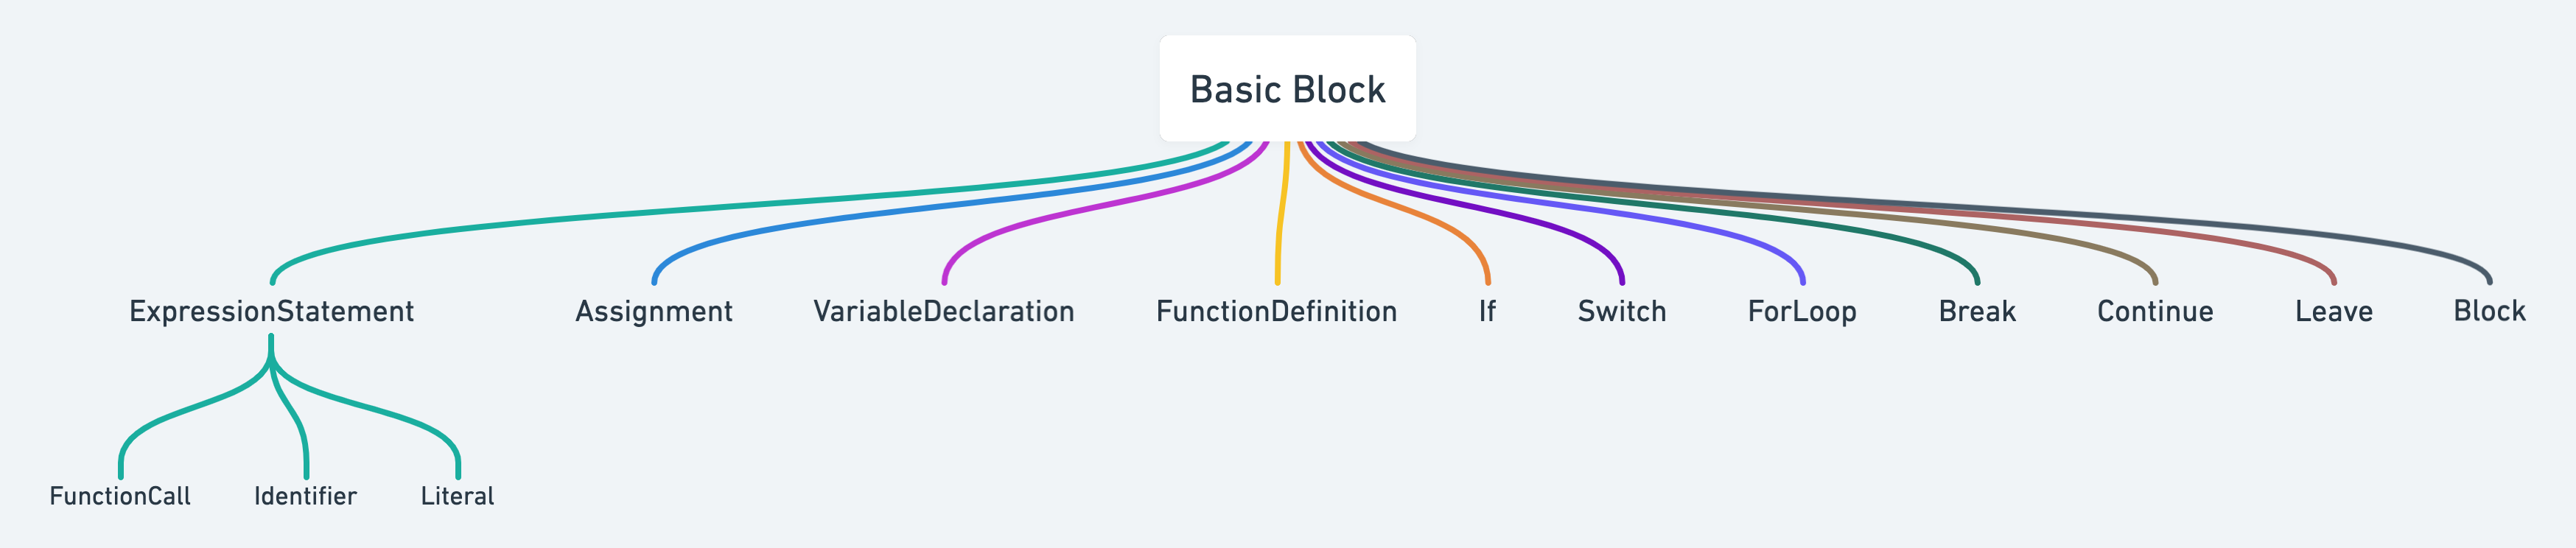
\includegraphics[width=\textwidth]{images/yul_ast_node_types.png}
    \caption{Node types in the YUL AST. Node properties vary depending on their nature.}
    \label{fig:yul-ast-node-types}
\end{figure}


\section{Other tools performing static analysis}
\paragraph*{}
The compiler has the option of outputting the Solidity AST in JSON format, which means that external tools can be built to alter the AST in any desired way. Since the compiler also supports receiving an AST as input, and generate bytecode from that one, that means that in theory one could build a better optimizer than the official one. While that hasn't happened yet, there are a few tools that perform code analysis of their own.

\subsection{Solidity Instrumentation Framework (SIF)}

Built by Chao Peng, Sefa Akca and Ajitha Rajan, from University of Edinburgh, SIF is a tool built in C that gravitates around the Visitor Design Pattern. The main objective is to build an internal C representation of Solidity code, through intermediary data structures, upon which SIF can orchestrate various optimizations / refactoring functions. As the authors describe it, it's a tool \cite[to easily and effectively understand, manipulate and analyse Solidity code]{sif}.

\begin{figure}
    \centering
    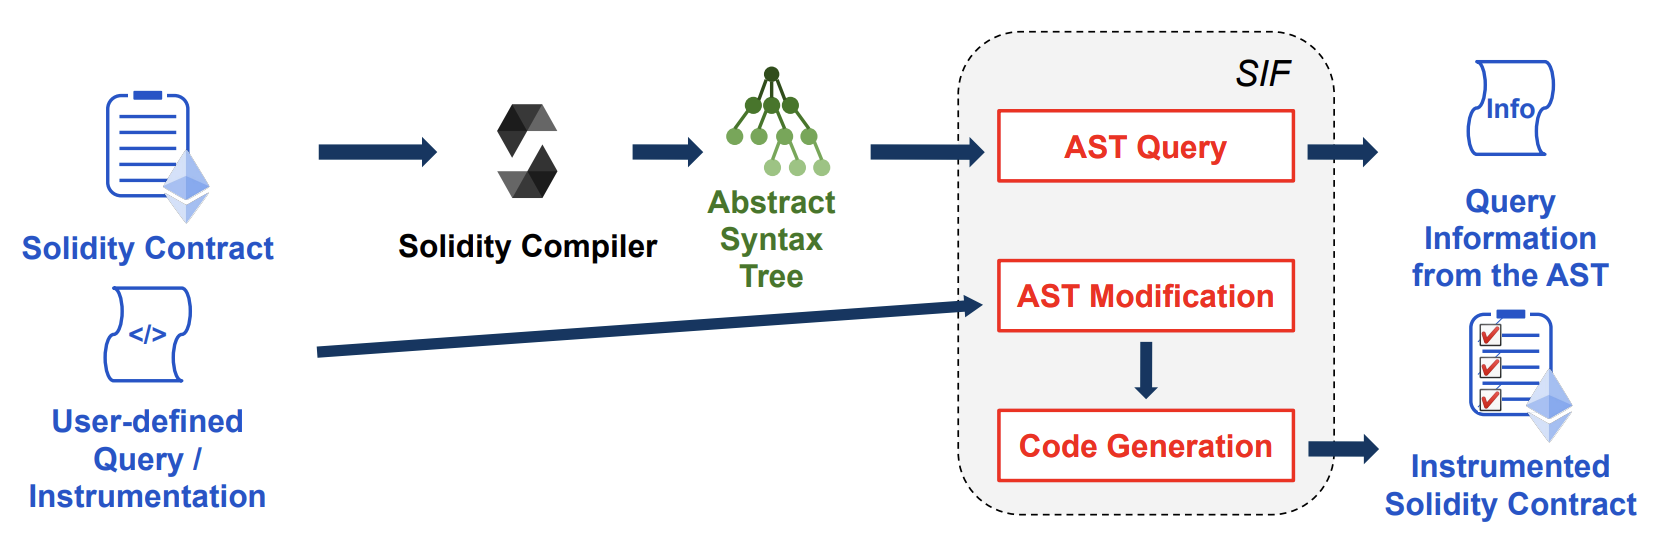
\includegraphics[width=15cm]{images/sif_workflow.png}
    \caption{SIF workflow, captured from SIF: A Framework for Solidity Contract Instrumentation and Analysis \cite{sif}}
    \label{fig:sif-workflow}
\end{figure}

The drawbacks that this toolkit currently has is that it's outdated and that it does not allow for external users to "plug-in" their own intermediate representations of Solidity code. It acts more as a middle-man, allowing users to implement, through the \emph{visit} method, specific optimization / refactoring items that run against isolated pieces of code. The tool does build a Control Flow Graph for the code, the one that this thesis will focus on, but it does not specifically use it for any kind of in-house optimization - it is just available to the user for usage. However, the completeness of the internal control flow graph is questionable.

\subsection{Slither}
\paragraph*{}
Slither is a more abstract, high level static analysis framework, which gives a broader overview over the internals of an Ethereum smart contract. Its main focus is centered around 4 areas: security (vulnerability detection), automated code optimization, code analysis and assisted code review, as described in Section 4.1 by the author Margherita Renieri \cite{slither}.

The tool takes advantage of the Abstract Syntax Tree (AST) built by the Solidity Compiler, then passes that through a series of optimization steps: Information Recovery, SlithIR Conversion and Code Analysis.

What's common in both of the tools we've seen is the usage of Abstract Syntax Trees and Control Flow Graphs, as well as building "proprietary" intermediate representation of the input code.

\begin{figure}
    \centering
    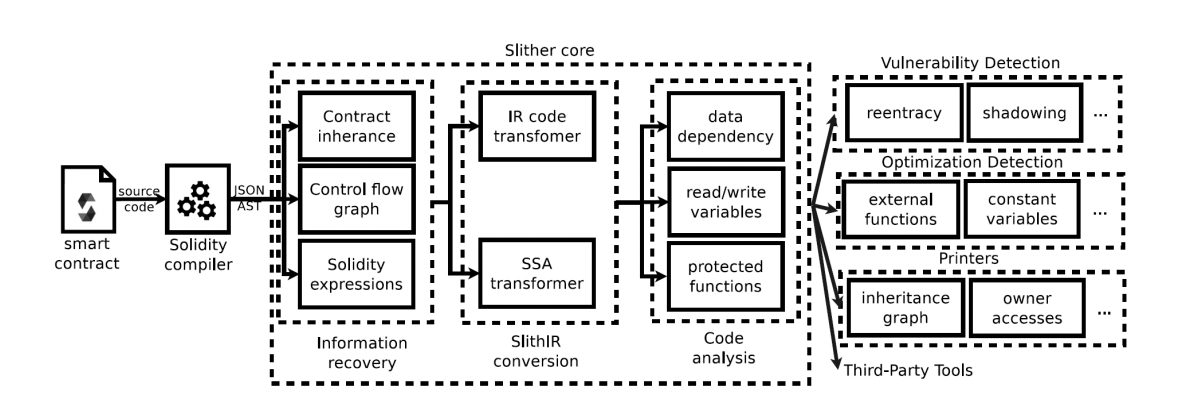
\includegraphics[width=15cm]{images/slither_architecture.png}
    \caption{Slither Architecture}
    \label{fig:slither-architecture}
\end{figure}

\subsection{Why focus on the official optimizer}
\paragraph*{}
The issue with such tools as SIF or Slither is that they get rapidly deprecated, since Solidity ground is so volatile, and they don't provide better optimization flows than Solidity's compiler does. Furthermore, integration is a bit more difficult, since it requires a separate optimization pipeline to be run through this intermediary tools, which just adds an additional burden to generating efficient bytecode.

What is certain is that the official compiler and optimizer will stay at the core of generating the Solidity bytecode. Therefore, any improvements to that will reflect itself in the next Solidity release - given it passes the team's rigurous reviews, of course.